\documentclass{standalone}
\usepackage{tikz}
\usetikzlibrary{patterns, positioning}
\usepackage[sfdefault]{ClearSans} %% option 'sfdefault' activates Clear Sans as the default text font
\usepackage[T1]{fontenc}

\begin{document}
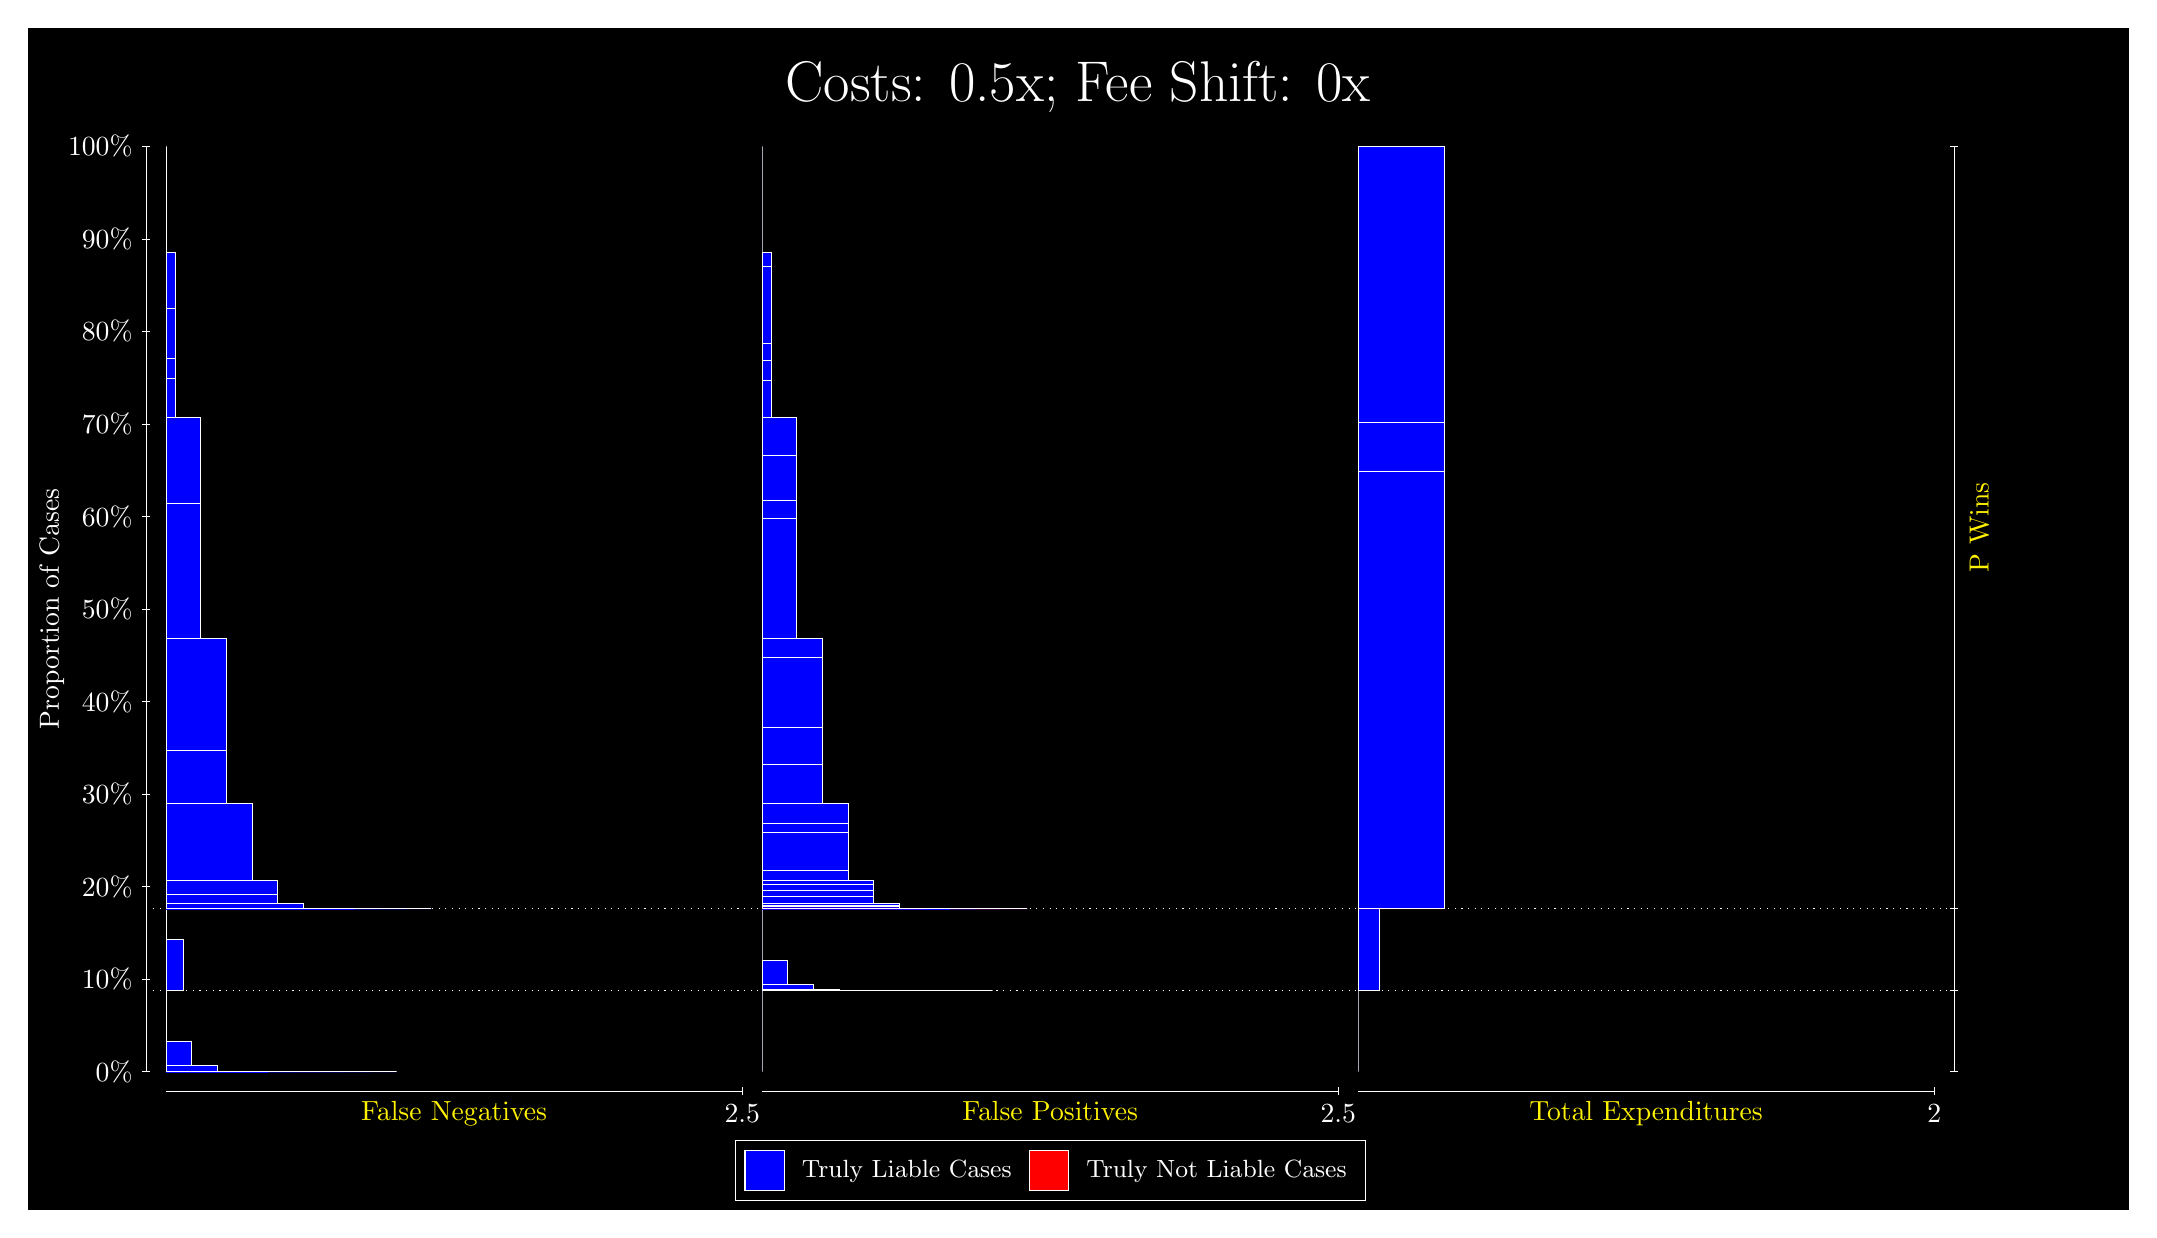
\begin{tikzpicture}
\draw[fill=black] (0,0) rectangle (26.667,15);
\draw[text=white] (0,13.5) rectangle (26.667,15) node[midway] {\huge Costs: 0.5x; Fee Shift: 0x};
\draw[white, very thin] (1.5,1.75) -- (1.5,13.5);
\node[rotate=90, text=white, anchor=center] at (0.3, 7.625) {Proportion of Cases};
\draw[white, very thin] (1.45,1.75) -- (1.55,1.75);
\node[text=white, anchor=east] at (1.45, 1.75) {0\%};
\draw[white, very thin] (1.45,2.925) -- (1.55,2.925);
\node[text=white, anchor=east] at (1.45, 2.925) {10\%};
\draw[white, very thin] (1.45,4.1) -- (1.55,4.1);
\node[text=white, anchor=east] at (1.45, 4.1) {20\%};
\draw[white, very thin] (1.45,5.275) -- (1.55,5.275);
\node[text=white, anchor=east] at (1.45, 5.275) {30\%};
\draw[white, very thin] (1.45,6.45) -- (1.55,6.45);
\node[text=white, anchor=east] at (1.45, 6.45) {40\%};
\draw[white, very thin] (1.45,7.625) -- (1.55,7.625);
\node[text=white, anchor=east] at (1.45, 7.625) {50\%};
\draw[white, very thin] (1.45,8.8) -- (1.55,8.8);
\node[text=white, anchor=east] at (1.45, 8.8) {60\%};
\draw[white, very thin] (1.45,9.975) -- (1.55,9.975);
\node[text=white, anchor=east] at (1.45, 9.975) {70\%};
\draw[white, very thin] (1.45,11.15) -- (1.55,11.15);
\node[text=white, anchor=east] at (1.45, 11.15) {80\%};
\draw[white, very thin] (1.45,12.325) -- (1.55,12.325);
\node[text=white, anchor=east] at (1.45, 12.325) {90\%};
\draw[white, very thin] (1.45,13.5) -- (1.55,13.5);
\node[text=white, anchor=east] at (1.45, 13.5) {100\%};

\draw[white, very thin] (24.457,1.75) -- (24.457,13.5);
\draw[white, very thin] (24.407,1.75) -- (24.507,1.75);
\node[anchor=west] at (24.407, 1.75) {};
\draw[white, very thin] (24.407,2.784) -- (24.507,2.784);
\node[anchor=west] at (24.407, 2.784) {};
\draw[white, very thin] (24.407,3.8181) -- (24.507,3.8181);
\node[anchor=west] at (24.407, 3.8181) {};
\draw[white, very thin] (24.407,13.5) -- (24.507,13.5);
\node[anchor=west] at (24.407, 13.5) {};

\draw[white, very thin, fill=blue] (1.75,1.75) rectangle (4.6775,1.75);
\draw[white, very thin, fill=blue] (1.75,1.75) rectangle (4.3523,1.75);
\draw[white, very thin, fill=blue] (1.75,1.75) rectangle (4.027,1.75);
\draw[white, very thin, fill=blue] (1.75,1.75) rectangle (3.7017,1.75);
\draw[white, very thin, fill=blue] (1.75,1.75) rectangle (3.3764,1.75);
\draw[white, very thin, fill=blue] (1.75,1.75) rectangle (3.0511,1.7503);
\draw[white, very thin, fill=blue] (1.75,1.7503) rectangle (2.7258,1.7573);
\draw[white, very thin, fill=blue] (1.75,1.7573) rectangle (2.4006,1.8289);
\draw[white, very thin, fill=blue] (1.75,1.8289) rectangle (2.0753,2.1333);
\draw[white, very thin, fill=red] (1.75,2.1333) rectangle (1.75,2.1333);
\draw[white, very thin, fill=blue] (1.75,2.1333) rectangle (1.75,2.784);
\draw[white, very thin, fill=blue] (1.75,2.784) rectangle (1.9696,3.4347);
\draw[white, very thin, fill=red] (1.75,3.4347) rectangle (1.75,3.4347);
\draw[white, very thin, fill=blue] (1.75,3.4347) rectangle (1.75,3.8181);
\draw[white, very thin, fill=blue] (1.75,3.8181) rectangle (5.1167,3.8181);
\draw[white, very thin, fill=blue] (1.75,3.8181) rectangle (4.7914,3.8181);
\draw[white, very thin, fill=blue] (1.75,3.8181) rectangle (4.7914,3.8181);
\draw[white, very thin, fill=blue] (1.75,3.8181) rectangle (4.4661,3.8181);
\draw[white, very thin, fill=blue] (1.75,3.8181) rectangle (4.4661,3.8181);
\draw[white, very thin, fill=blue] (1.75,3.8181) rectangle (4.1408,3.8186);
\draw[white, very thin, fill=blue] (1.75,3.8186) rectangle (3.8155,3.8225);
\draw[white, very thin, fill=blue] (1.75,3.8225) rectangle (3.8155,3.8252);
\draw[white, very thin, fill=blue] (1.75,3.8252) rectangle (3.4903,3.8807);
\draw[white, very thin, fill=blue] (1.75,3.8807) rectangle (3.165,4.0009);
\draw[white, very thin, fill=blue] (1.75,4.0009) rectangle (3.165,4.1745);
\draw[white, very thin, fill=blue] (1.75,4.1745) rectangle (2.8397,5.1607);
\draw[white, very thin, fill=blue] (1.75,5.1607) rectangle (2.5144,5.8282);
\draw[white, very thin, fill=blue] (1.75,5.8282) rectangle (2.5144,7.2539);
\draw[white, very thin, fill=blue] (1.75,7.2539) rectangle (2.1891,8.9662);
\draw[white, very thin, fill=blue] (1.75,8.9662) rectangle (2.1891,10.064);
\draw[white, very thin, fill=blue] (1.75,10.064) rectangle (1.8638,10.556);
\draw[white, very thin, fill=blue] (1.75,10.556) rectangle (1.8638,10.805);
\draw[white, very thin, fill=blue] (1.75,10.805) rectangle (1.8638,11.443);
\draw[white, very thin, fill=blue] (1.75,11.443) rectangle (1.8638,12.157);
\draw[white, very thin, fill=red] (1.75,12.157) rectangle (1.75,12.157);
\draw[white, very thin, fill=blue] (1.75,12.157) rectangle (1.75,13.5);
\draw[white, very thin, fill=red] (9.3189,1.75) rectangle (9.3189,1.75);
\draw[white, very thin, fill=blue] (9.3189,1.75) rectangle (9.3189,2.784);
\draw[white, very thin, fill=red] (9.3189,2.784) rectangle (12.246,2.784);
\draw[white, very thin, fill=blue] (9.3189,2.784) rectangle (12.246,2.784);
\draw[white, very thin, fill=blue] (9.3189,2.784) rectangle (11.921,2.784);
\draw[white, very thin, fill=blue] (9.3189,2.784) rectangle (11.596,2.784);
\draw[white, very thin, fill=blue] (9.3189,2.784) rectangle (11.271,2.784);
\draw[white, very thin, fill=blue] (9.3189,2.784) rectangle (10.945,2.784);
\draw[white, very thin, fill=blue] (9.3189,2.784) rectangle (10.62,2.7843);
\draw[white, very thin, fill=blue] (9.3189,2.7843) rectangle (10.295,2.7913);
\draw[white, very thin, fill=blue] (9.3189,2.7913) rectangle (9.9694,2.863);
\draw[white, very thin, fill=blue] (9.3189,2.863) rectangle (9.6442,3.1673);
\draw[white, very thin, fill=blue] (9.3189,3.1673) rectangle (9.3189,3.8181);
\draw[white, very thin, fill=red] (9.3189,3.8181) rectangle (12.686,3.8181);
\draw[white, very thin, fill=blue] (9.3189,3.8181) rectangle (12.686,3.8181);
\draw[white, very thin, fill=red] (9.3189,3.8181) rectangle (12.36,3.8181);
\draw[white, very thin, fill=blue] (9.3189,3.8181) rectangle (12.36,3.8181);
\draw[white, very thin, fill=red] (9.3189,3.8181) rectangle (12.035,3.8181);
\draw[white, very thin, fill=blue] (9.3189,3.8181) rectangle (12.035,3.8181);
\draw[white, very thin, fill=blue] (9.3189,3.8181) rectangle (12.035,3.8181);
\draw[white, very thin, fill=blue] (9.3189,3.8181) rectangle (12.035,3.8181);
\draw[white, very thin, fill=red] (9.3189,3.8181) rectangle (11.71,3.8181);
\draw[white, very thin, fill=blue] (9.3189,3.8181) rectangle (11.71,3.8184);
\draw[white, very thin, fill=blue] (9.3189,3.8184) rectangle (11.71,3.8186);
\draw[white, very thin, fill=red] (9.3189,3.8186) rectangle (11.384,3.8186);
\draw[white, very thin, fill=blue] (9.3189,3.8186) rectangle (11.384,3.821);
\draw[white, very thin, fill=blue] (9.3189,3.821) rectangle (11.384,3.8252);
\draw[white, very thin, fill=blue] (9.3189,3.8252) rectangle (11.059,3.8439);
\draw[white, very thin, fill=red] (9.3189,3.8439) rectangle (11.059,3.8439);
\draw[white, very thin, fill=blue] (9.3189,3.8439) rectangle (11.059,3.8608);
\draw[white, very thin, fill=blue] (9.3189,3.8608) rectangle (11.059,3.8807);
\draw[white, very thin, fill=blue] (9.3189,3.8807) rectangle (10.734,3.9694);
\draw[white, very thin, fill=blue] (9.3189,3.9694) rectangle (10.734,4.0535);
\draw[white, very thin, fill=red] (9.3189,4.0535) rectangle (10.734,4.0535);
\draw[white, very thin, fill=blue] (9.3189,4.0535) rectangle (10.734,4.1298);
\draw[white, very thin, fill=blue] (9.3189,4.1298) rectangle (10.734,4.1745);
\draw[white, very thin, fill=blue] (9.3189,4.1745) rectangle (10.409,4.3053);
\draw[white, very thin, fill=red] (9.3189,4.3053) rectangle (10.409,4.3053);
\draw[white, very thin, fill=blue] (9.3189,4.3053) rectangle (10.409,4.7868);
\draw[white, very thin, fill=blue] (9.3189,4.7868) rectangle (10.409,4.9015);
\draw[white, very thin, fill=blue] (9.3189,4.9015) rectangle (10.409,5.1607);
\draw[white, very thin, fill=blue] (9.3189,5.1607) rectangle (10.083,5.6573);
\draw[white, very thin, fill=blue] (9.3189,5.6573) rectangle (10.083,6.1241);
\draw[white, very thin, fill=red] (9.3189,6.1241) rectangle (10.083,6.1241);
\draw[white, very thin, fill=blue] (9.3189,6.1241) rectangle (10.083,7.0097);
\draw[white, very thin, fill=blue] (9.3189,7.0097) rectangle (10.083,7.254);
\draw[white, very thin, fill=blue] (9.3189,7.254) rectangle (9.758,8.7815);
\draw[white, very thin, fill=red] (9.3189,8.7815) rectangle (9.758,8.7815);
\draw[white, very thin, fill=blue] (9.3189,8.7815) rectangle (9.758,8.9986);
\draw[white, very thin, fill=blue] (9.3189,8.9986) rectangle (9.758,9.5768);
\draw[white, very thin, fill=blue] (9.3189,9.5768) rectangle (9.758,10.064);
\draw[white, very thin, fill=blue] (9.3189,10.064) rectangle (9.4327,10.531);
\draw[white, very thin, fill=blue] (9.3189,10.531) rectangle (9.4327,10.78);
\draw[white, very thin, fill=blue] (9.3189,10.78) rectangle (9.4327,10.998);
\draw[white, very thin, fill=blue] (9.3189,10.998) rectangle (9.4327,11.982);
\draw[white, very thin, fill=blue] (9.3189,11.982) rectangle (9.4327,12.157);
\draw[white, very thin, fill=blue] (9.3189,12.157) rectangle (9.3189,13.5);
\draw[white, very thin, fill=red] (16.888,1.75) rectangle (16.888,1.75);
\draw[white, very thin, fill=blue] (16.888,1.75) rectangle (16.888,2.784);
\draw[white, very thin, fill=red] (16.888,2.784) rectangle (17.162,2.784);
\draw[white, very thin, fill=blue] (16.888,2.784) rectangle (17.162,3.8181);
\draw[white, very thin, fill=red] (16.888,3.8181) rectangle (17.986,3.8181);
\draw[white, very thin, fill=blue] (16.888,3.8181) rectangle (17.986,9.3736);
\draw[white, very thin, fill=red] (16.888,9.3736) rectangle (17.986,9.3736);
\draw[white, very thin, fill=blue] (16.888,9.3736) rectangle (17.986,9.9936);
\draw[white, very thin, fill=red] (16.888,9.9936) rectangle (17.986,9.9936);
\draw[white, very thin, fill=blue] (16.888,9.9936) rectangle (17.986,13.5);
\draw[white, dotted] (1.5,2.784) -- (24.457,2.784);
\draw[white, dotted] (1.5,3.8181) -- (24.457,3.8181);
\draw[white, very thin] (1.75,1.5) -- (9.0689,1.5);
\node[text=yellow, anchor=north] at (5.4094, 1.5) {False Negatives};
\draw[white, very thin] (9.0689,1.45) -- (9.0689,1.55);
\node[text=white, anchor=north] at (9.0689, 1.45) {2.5};

\draw[white, very thin] (9.3189,1.5) -- (16.638,1.5);
\node[text=yellow, anchor=north] at (12.978, 1.5) {False Positives};
\draw[white, very thin] (16.638,1.45) -- (16.638,1.55);
\node[text=white, anchor=north] at (16.638, 1.45) {2.5};

\draw[white, very thin] (16.888,1.5) -- (24.207,1.5);
\node[text=yellow, anchor=north] at (20.547, 1.5) {Total Expenditures};
\draw[white, very thin] (24.207,1.45) -- (24.207,1.55);
\node[text=white, anchor=north] at (24.207, 1.45) {2};



\node[text=yellow, centered, rotate=90] at (24.777, 8.659) {P Wins};

\draw (12.978300999999998,1.5) node[draw=none] (baseCoordinate) {};
\begin{scope}[align=center]
        \matrix[scale=0.5, draw=white, below=0.5cm of baseCoordinate, nodes={draw}, column sep=0.1cm]{
            \node[rectangle, draw, minimum width=0.5cm, minimum height=0.5cm, fill=blue] {}; &
            \node[draw=none, font=\small, text=white] (B) {Truly Liable Cases}; &
            \node[rectangle, draw, minimum width=0.5cm, minimum height=0.5cm, fill=red] {}; &
            \node[draw=none, font=\small, text=white] (B) {Truly Not Liable Cases}; \\
            };
\end{scope}

\end{tikzpicture}
\end{document}